\documentclass[a4paper, 12pt]{article}%тип документа

%отступы
\usepackage[left=1.5cm,right=1cm,top=2cm,bottom=3cm,bindingoffset=0cm]{geometry}
\setlength{\parindent}{5ex}

%Русский язык
\usepackage[T2A]{fontenc} %кодировка
\usepackage[utf8]{inputenc} %кодировка исходного кода
\usepackage[english,russian]{babel} %локализация и переносы

%Вставка картинок
\usepackage{graphicx}
\graphicspath{{pictures/}}
\DeclareGraphicsExtensions{.pdf,.png,.jpg,}
\usepackage{wrapfig}

%Графики
\usepackage{pgfplots}
\pgfplotsset{compat=1.9}

%Математика
\usepackage{amsmath, amsfonts, amssymb, amsthm, mathtools}

%Таблицы
\usepackage{longtable} 
\usepackage{float}

%Римские цифры
\newcommand{\RomanNumeralCaps}[1]{\uppercase\expandafter{\romannumeral#1}}

\usepackage{multirow}



\begin{document}
	\begin{titlepage}
		\begin{center}
			\textsc{Федеральное государственное автономное образовательное учреждение высшего образования«Московский физико-технический институт (национальный исследовательский университет)»\\[5mm]
			}
			
			\vfill
			
			\textbf{Отчёт по лабораторной работе 5.2.1\\[3mm]
				Опыт Франка-Герца
				\\[50mm]
			}
			
		\end{center}
		
		\hfill
		\begin{minipage}{.5\textwidth}
			Выполнили студенты:\\[2mm]
			Сериков Василий Романович\\[2mm]
			Сериков Алексей Романович\\[2mm]
			группа: Б03-102\\[5mm]
			
		\end{minipage}
		\vfill
		\begin{center}
			Москва, 2023 г.
		\end{center}
		
	\end{titlepage}
	
	\newpage
	\setcounter{page}{2}
	\textbf{Аннотация}\\
	
	\textbf{Цель работы: }\\
Методом электронного возбуждения измерить энергии первого уровня атома гелия в динамическом и статическом режимах.\\

	\textbf{Теория}\\
Одним из простых опытов, подтверждающих существование дискретных уровней энергии атомов, является эксперимент Франка и Герца.

Разреженный одноатомный газ заполняет трехэлектродную лампу.  Электроны, испускаемые разогретым катодом, ускоряются в постоянном электрическом поле, созданным между катодом и сетчатым анодом лампы. Передвигаясь от катода к аноду, электроны сталкиваются с атомами гелия. Если энергия электрона, налетающего на атом, недостаточна для того, чтобы перевести его в возбуждённое состояние (или ионизовать), то возможны только упругие соударения, при которых электроны почти не теряют энергии, так как их масса в тысячи раз меньше массы атомов.

При увеличении напряжения на электродах увеличивается энергия электронов и оказывается достаточной для возбуждения атомов, при этом ток коллектора резко уменьшается. При дальнейшем увеличении потенциала анода ток коллектора возрастает, электроны, испытавшие неупругие соударения набирают энергию, достаточную для преодоления задерживающего потенциала.

\begin{figure}[H]
	\centering
	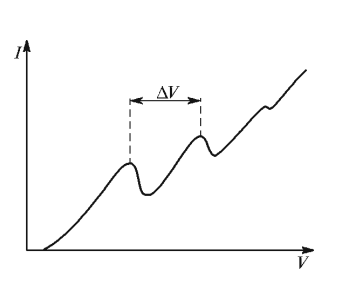
\includegraphics[width=0.6\linewidth]{1}
	\caption{Схематический вид зависимости тока коллектора от напряжения на аноде}
\end{figure}


\textbf{Экспериментальная установка}\\

Схема экспериментальной установки изображена на рис.2

Источником электронов является вольфрамовый катод, нагреваемы переменным током. В качестве анода используется двойная спираль, окружающая катод. Коллектор - полый цилиндр, соосный с катодом и анодом.  

\begin{figure}[H]
	\centering
	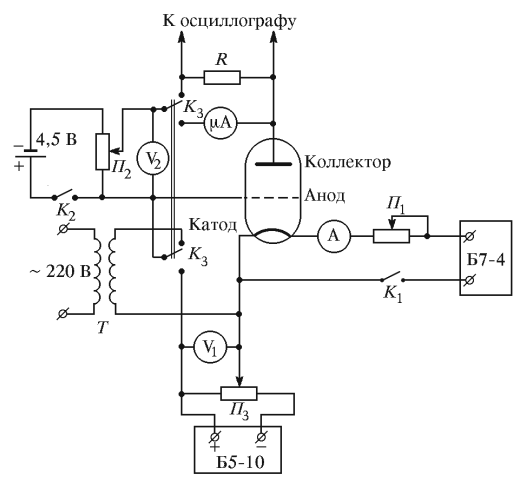
\includegraphics[width=0.6\linewidth]{ust}
	\caption{Схематический вид зависимости тока коллектора от напряжения на аноде}
\end{figure}


	\textbf{Ход работы: }\\
	\begin{enumerate}
	

	\item При максимальном ускоряющем напряжении измерим на экране осциллографа расстояние между максимумами и расстояние межу минимумами осциллограммы. Результаты занесем в таблицу 1. Сфотографируем осциллограммы для трех значений задерживающего напряжения: 4В, 6В, 8В. Полученные фото изобразим на рисунках 1-3.
	
	\begin{figure}[H]
		\centering
		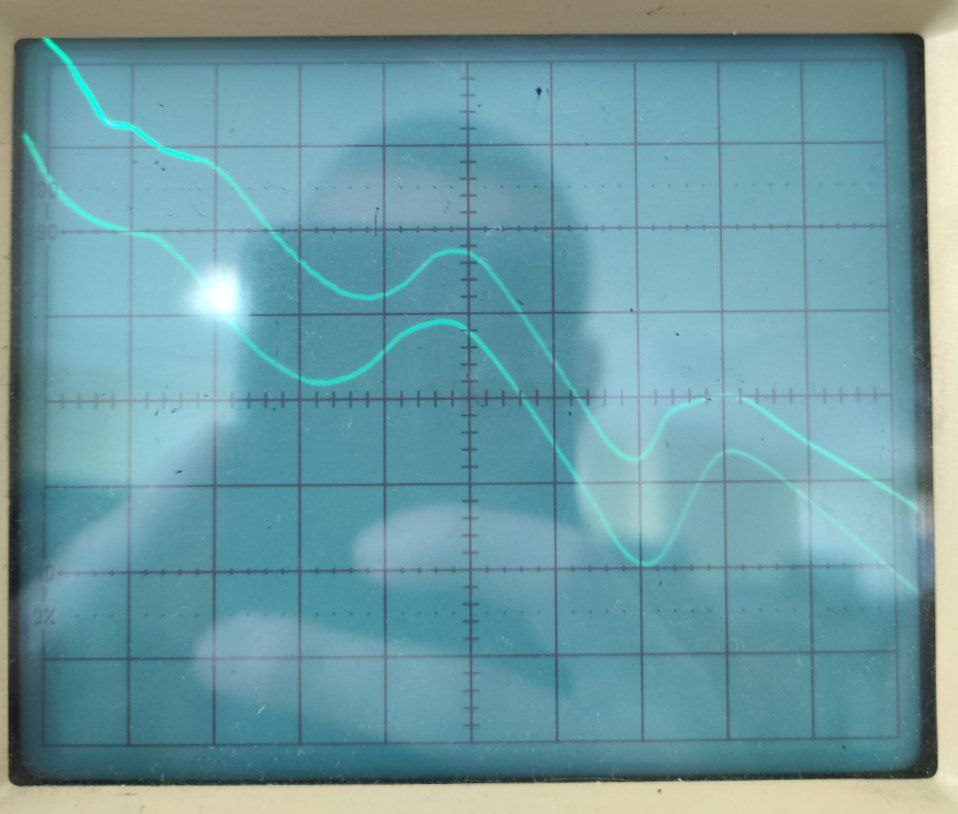
\includegraphics[width=0.6\linewidth]{4v_}
		\caption{Осциллограмма полученная для запирающего напряжения 4В}
	\end{figure}

	\begin{figure}[H]
		\centering
		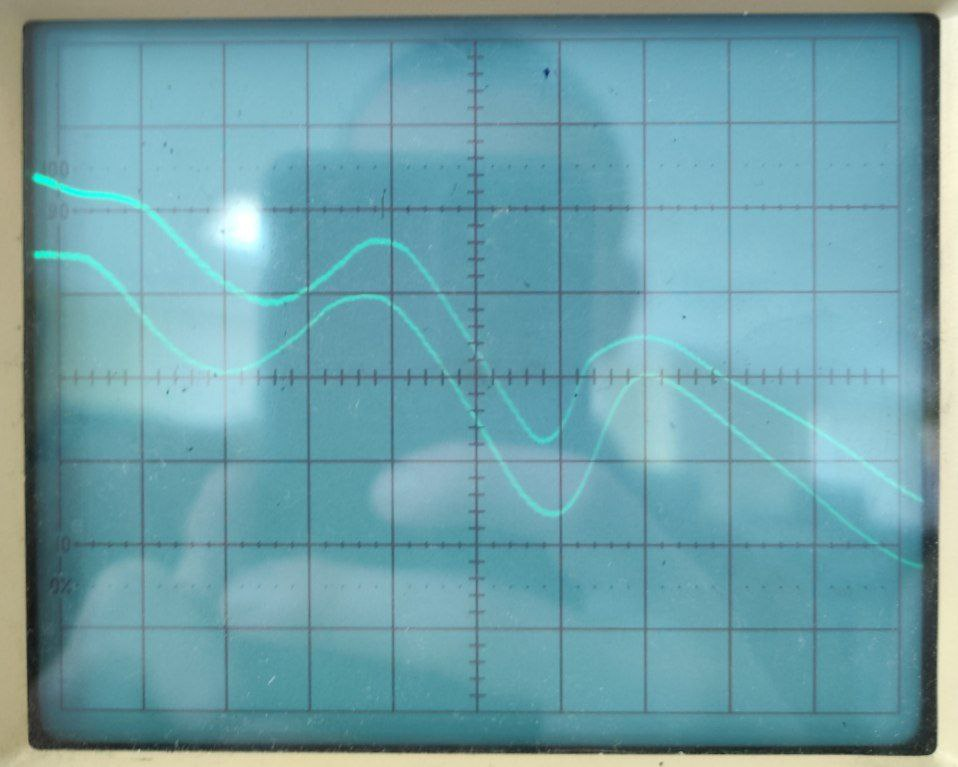
\includegraphics[width=0.6\linewidth]{6v_}
		\caption{Осциллограмма полученная для запирающего напряжения 6В}
	\end{figure}

	\begin{figure}[H]
		\centering
		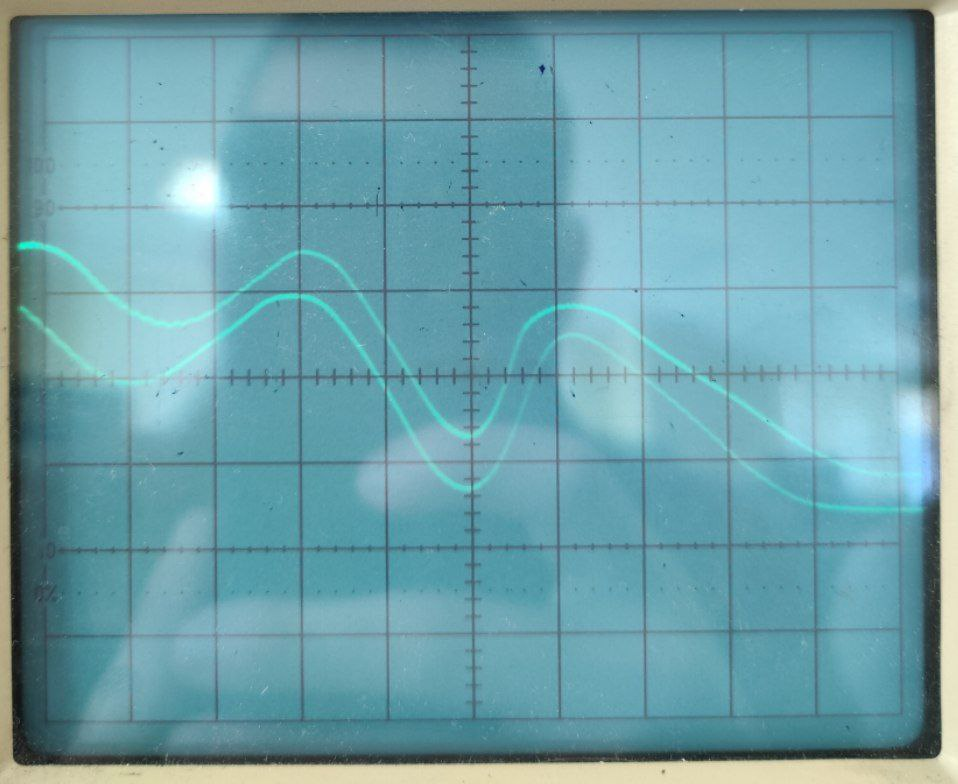
\includegraphics[width=0.6\linewidth]{8v_}
		\caption{Осциллограмма полученная для запирающего напряжения 8В}
	\end{figure}
	
	\begin{longtable}{|c|c|c|c|c|c|c|}
		\hline
		$V_\text{зап.},$ В & $\Delta V_{max}, $ Дел. & $\Delta V_{min}, $ Дел. & $\sigma_{\Delta V_{max/min}}, $ Дел. & $\Delta V_{max}, $ В & $\Delta V_{min}, $ В& $\sigma_{\Delta V_{max/min}}, $ В\\ \hline
		4 & 3,4 & 3,9 & \multirow{3}{*}{0,2} & 17 & 20 & \multirow{3}{*}{1}\\ \cline{1-3} \cline{5-6}
		6 & 3,4 & 3,9 &                    & 17 & 20   &  				   \\ \cline{1-3} \cline{5-6}
		8 & 3,2 & 3,8 &                    & 16 & 19     &                     \\ \hline
		\caption{Полученные результаты для расстояния между максимумами и минимумами на осциллограмме}
	\end{longtable} 
 
	 $$ \overline {\Delta V_{max}} = 17 \pm 1 \text{ В}  $$
	 
	 $$ \overline {\Delta V_{min}} = 20 \pm 1 \text{ В} $$
	 
	 $$ \overline {\Delta V} = 19 \pm 2\text{ В} $$
	 
	 \newpage
	 
	 Расчет погрешности  проводился по формулам:
	 
	 $$ \sigma_{\overline{\Delta V_{max/min}}} = \sqrt{\frac{1}{n(n-1)} \sum_{i = 1}^{n} (\overline{\Delta V} - \Delta {V_i})^2} $$
	 
	 $$ \sigma_{\Delta V} = \sqrt{ \sigma_{\overline{\Delta V_{max/min}}} ^2 + \sigma_{\Delta V_{max/min}}^2 }$$

	\item Снимем зависимость коллекторного тока от анодного напряжения $[I_k = f(V_a)]$ для трех различных значений запирающего напряжения $V_2$ = 4, 6, 8 В. Результаты измерений внесем в таблицу 2. По полученным данным построим графики зависимости $I_k = f(V_a)$
	

\newpage

\begin{longtable}{|c|c|c|c|c|c|}
	\hline
	$I_{k1},$ мА & $V_{a1}$, В & $I_{k2},$ мА & $V_{a2}$, В & $I_{k3},$ мА & $V_{a3}$, В  \\ \hline
	18,5 & 3,33 & 6,1 & 3,01 & 5,0 & 4,68 \\ \hline
	34,0 & 5,66 & 16,0 & 4,98 & 8,9 & 5,43 \\ \hline
	41,0 & 6,65 & 30,6 & 7,1 & 13,9 & 6,49 \\ \hline 
	45,8 & 7,31 & 43,5 & 8,88 & 31,3 & 8,93 \\ \hline 
	53,2 & 8,40 & 51,3 & 10,03 & 58,0 & 12,79 \\ \hline
	61,5 & 9,69 & 60,1 & 11,35 & 83,6 & 16,95 \\ \hline
	67,7 & 10,68 & 74,2 & 13,47 & 95,0 & 20,38 \\ \hline
	74,9 & 11,87 & 94,9 & 16,90 & 88,6 & 22,22 \\ \hline
	81,2 & 12,92 & 103,6 & 19,15 & 47,0 & 23,44 \\ \hline
	86,4 & 13,27 & 96,0 & 21,53 & 23,7 & 24,45 \\ \hline
	92,7 & 14,82 & 60,7 & 22,91 & 17,5 & 24,98 \\ \hline
	98,3 & 15,79 & 45,2 & 23,51 & 16,2 & 26,97 \\ \hline
	105,1 & 21,90 & 36,6 & 24,47 & 46,2 & 30,04 \\ \hline
	86,6 & 22,30 & 47,0 & 26,80 & 76,8 & 32,62 \\ \hline
	64,9 & 23,80 & 65,0 & 27,50 & 112,3 & 36,20 \\ \hline
	79,7 & 25,71 & 92,6 & 30,11 & 114,5 & 39,75 \\ \hline
	100,8 & 27,75 & 119,8 & 32,50 & 101,7 & 41,81 \\ \hline
	125,0 & 30,13 & 141,3 & 34,92 & 86,6 & 44,75 \\ \hline
	144,6 & 32,03 & 148,0 & 36,32 & 74,8 & 50,12 \\ \hline
	171,2 & 34,85 & 147,4 & 38,65 & 87,6 & 54,31 \\ \hline
	181,5 & 37,51 & 131,5 & 41,07 & 103,4 & 57,09 \\ \hline
	172,0 & 40,18 & 123,4 & 42,67 & 115,3 & 60,27 \\ \hline
	155,1 & 44,63 & 116,4 & 44,30 & 117,0 & 65,50 \\ \hline
	161,5 & 47,39 & 111,9 & 46,70 & 113,6 & 69,01 \\ \hline
	173,9 & 50,23 & 115,6 & 49,10 & 112,6 & 75,57 \\ \hline
	196,3 & 54,06 & 142,2 & 55,01 & 120,0 & 79,40 \\ \hline
	217,6 & 57,71 & 169,2 & 61,03 & 90,0 & 18,13 \\ \hline
	229,0 & 60,65 & 171,1 & 66,57 & 70,4 & 22,92 \\ \hline
	233,5 & 64,20 & 180,6 & 75,58 & 25,2 & 29,10 \\ \hline
	241,5 & 69,28 & 191,3 & 79,63 & 100,3 & 34,21 \\ \hline
	248,5 & 72,29 & 75,5 & 22,12 & 79,5 & 47,35 \\ \hline
	265,1 & 77,25 & 40,1 & 26,08 & 80,1 & 52,07 \\ \hline
	276,3 & 80,19 & 130,8 & 53,10 & 20,0 & 28,51 \\ \hline
	  
	108,5 & 18,01 & 175,2 & 72,31 & - & - \\ \hline
	111,2 & 20,43 & 155,1 & 53,15 & - & - \\ \hline
	95,2 & 22,13 & - & - & - & - \\ \hline
	75,3 & 23,18 & - & - & - & - \\ \hline
	90,1 & 26,82 & - & - & - & - \\ \hline
	161,3 & 42,02 & - & - & - & - \\ \hline
	
	\caption{Полученная зависимость $I_k = f(V_a)$. Индексам 1, 2, 3 сопоставлены значения напряжения $V_2$ = 4, 6, 8 В соответственно}
\end{longtable} 

\newpage

	\begin{figure}[H]
		\centering
		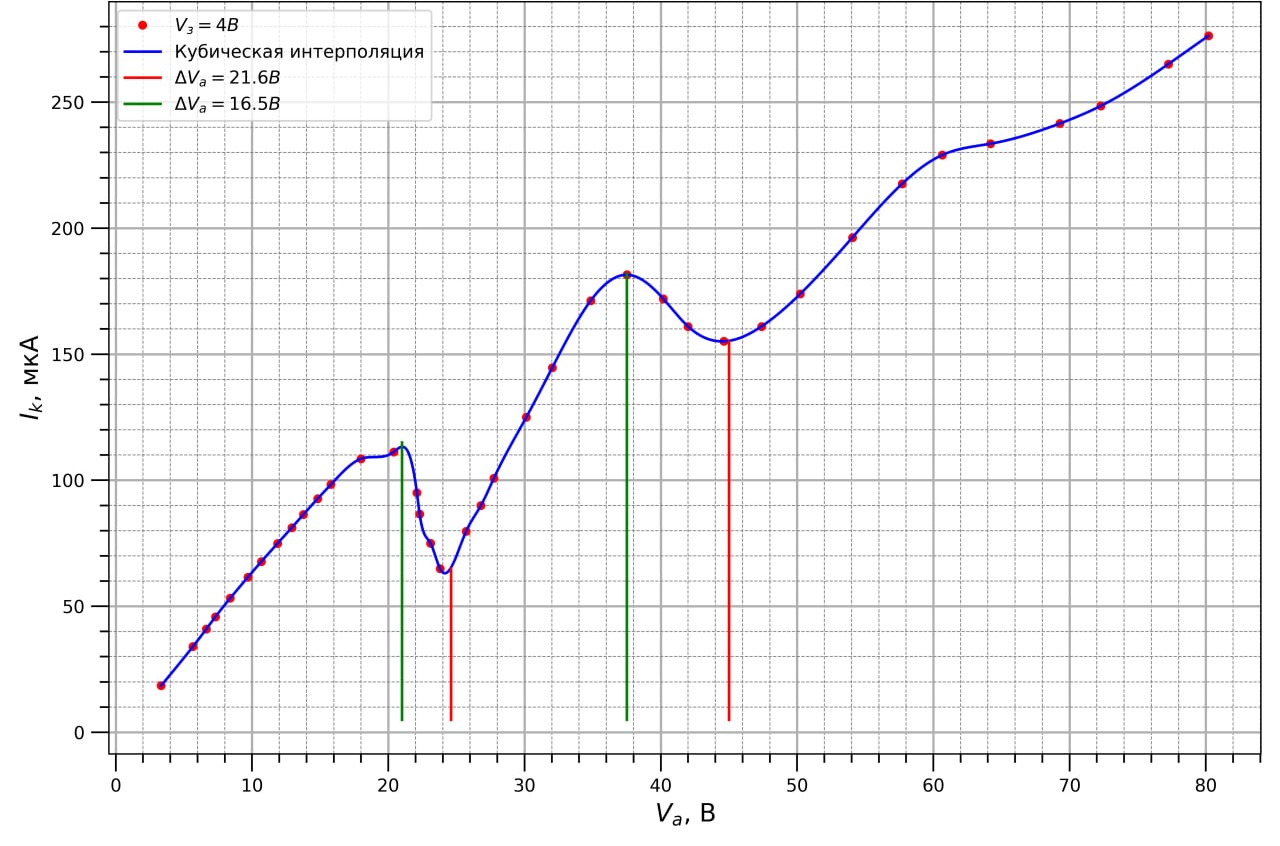
\includegraphics[width=1\linewidth]{4v}
		\caption{График зависимости коллекторного тока от анодного напряжения при запирающем напряжении 4В. Интерполяция кубическая}
	\end{figure}

	\begin{figure}[H]
		\centering
		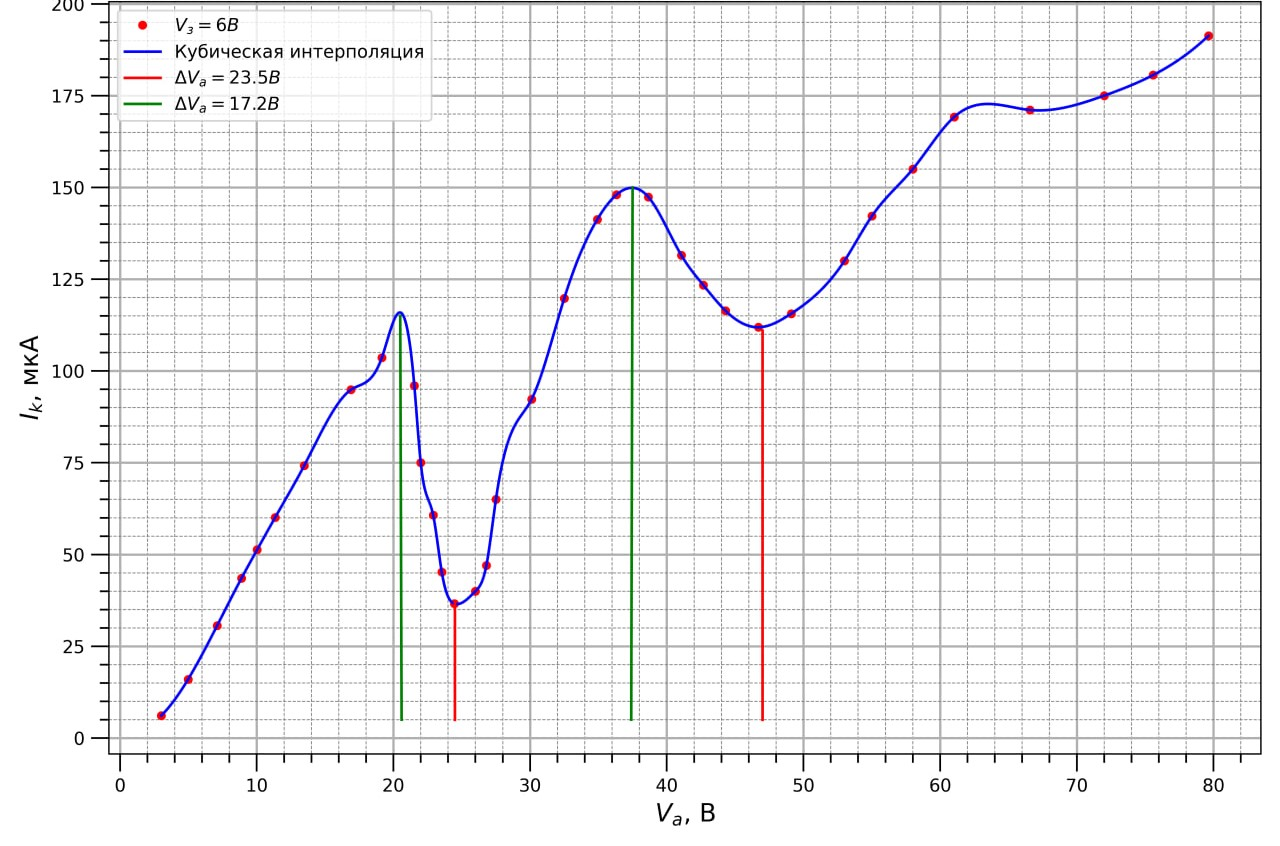
\includegraphics[width=1\linewidth]{6v}
		\caption{График зависимости коллекторного тока от анодного напряжения при запирающем напряжении 6В. Интерполяция кубическая}
	\end{figure}

	\begin{figure}[H]
		\centering
		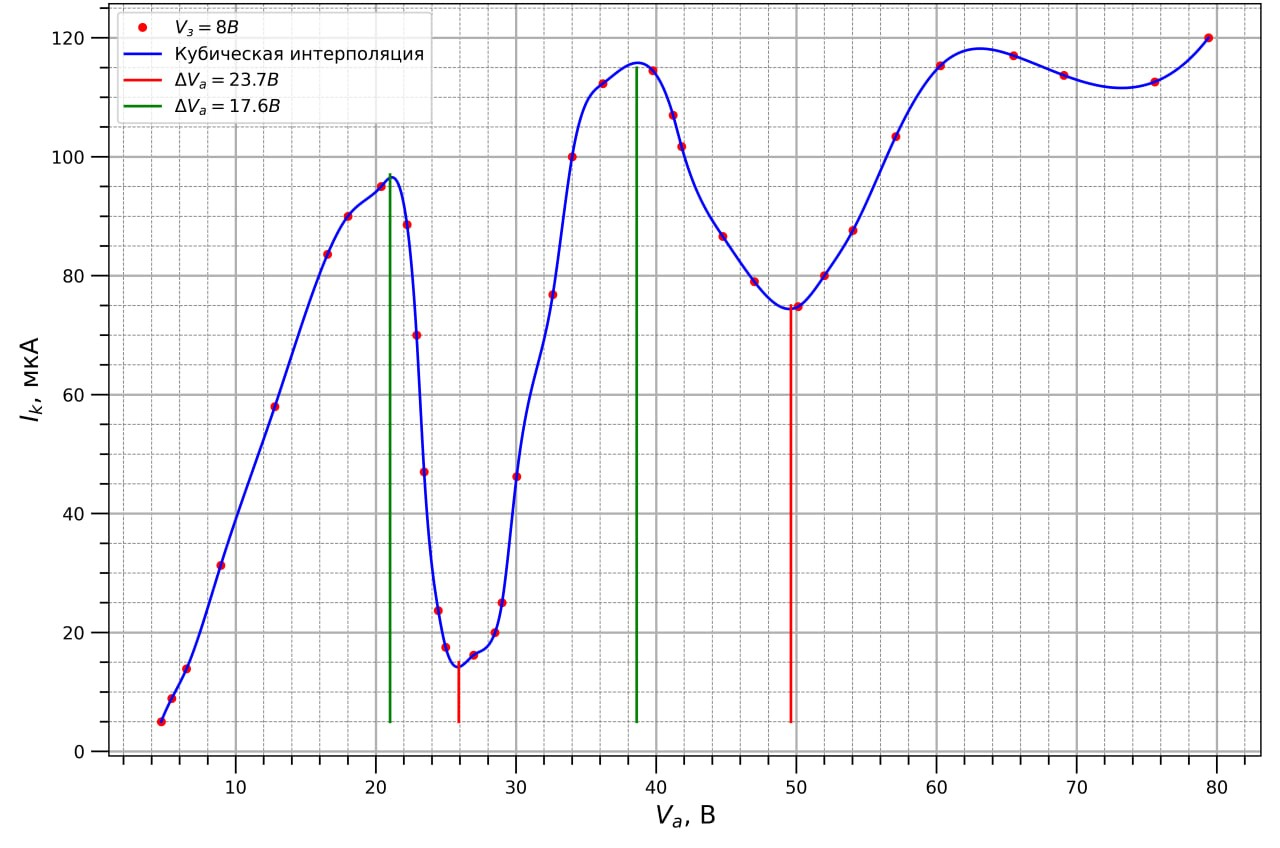
\includegraphics[width=1\linewidth]{8v}
		\caption{График зависимости коллекторного тока от анодного напряжения при запирающем напряжении 8В. Интерполяция кубическая}
	\end{figure}

	\newpage
 
	\item Определим по графикам разность напряжений $\Delta V_{max}$ и $\Delta V_{min}$ для каждого значения запирающего напряжения. Полученные данные запишем в таблицу 3.
 
	\begin{longtable}{|c|c|c|c|}
		\hline
		$V_\text{зап.},$ В  & $\Delta V_{max}, $ В & $\Delta V_{min}, $ В& $\sigma_{\Delta V_{max/min}}, $ В\\ \hline
		4  & 17 & 21 & \multirow{3}{*}{2}\\ \cline{1-3}
		6 & 18 & 23   &  				   \\ \cline{1-3}
		8 & 17 & 24     &                     \\ \hline
		\caption{Полученные результаты для расстояния между максимумами и минимумами по построенным графикам}
	\end{longtable}  

	 $$ \overline {\Delta V_{max}} = 17 \pm 2 \text{ В}  $$
	
	$$ \overline {\Delta V_{min}} = 23 \pm 2 \text{ В} $$
	
	$$ \overline {\Delta V} = 20 \pm 3\text{ В} $$
	
	Расчет погрешности  проводился по формулам из пункта 1\\
	
 \item По полученным напряжениям на осциллограммах и графиках определим энергию возбуждения первого уровня атома гелия. Результаты полученные статическим и динамическим методами занесем в таблицу 4.


	\begin{longtable}{|c|c|c|c|}
		\hline
	$\Delta V_{\text{стат.}}, $ В  & $\Delta V_{\text{дин.}}, $ В  & $E_{\text{стат.}}, $ эВ &  $E_{\text{дин.}}, $ эВ  \\ \hline
	
	19$\pm2$ & 20$\pm3$ & 19$\pm2$ & 20$\pm3$ \\ \hline

		\caption{Полученные результаты динамическим и статическим методами для энергии возбуждения первого уровня атома гелия}
	\end{longtable}  

	\end{enumerate}

	\textbf{Обсуждение результатов и выводы: }\\

	В ходе данной работы мы с помощью метода электронного возбуждения измерили энергию первого уровня атома гелия в динамическом и статическом режимах. Полученные данные совпадают в пределах погрешности с табличным значением $E_{\text{теор.}} $ = 20,8 эВ. Табличные данные изображены на рисунке 6.
	
	Основной вклад в погрешность полученных результатов для обоих методов дают погрешности измерения. В первом случае это погрешность цены деления шкалы на осциллографе, во втором погрешность из-за малого количества точек на графиках. Можно попытаться уменьшить эти погрешности, если использовать другую развертку на осциллографе, при которой на экране будет помещаться только два пика или два минимума, а не вся картина целиком. В статическом случае можно уменьшить погрешность, если снять бОльшее количество точек, тогда интерполяция будет точнее описывать истинную зависимость  $I_k = f(V_a)$ и получиться установить максимумы и минимумы точнее, использую более мелкую сетку.
	
	\begin{figure}[H]
		\centering
		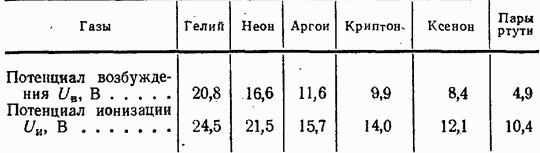
\includegraphics[width= 0.8 \linewidth]{E_ion}
		\caption{}
	\end{figure}
 
 
 \end{document}